\chapter{Figuren}
\section{Bild}
Bildern können Unterschriften hinzugefügt werden. Außerdem kann auf die bilder verwiesen werden (siehe \autoref{fig:image1})
\begin{figure}[htbp]
	\centering
	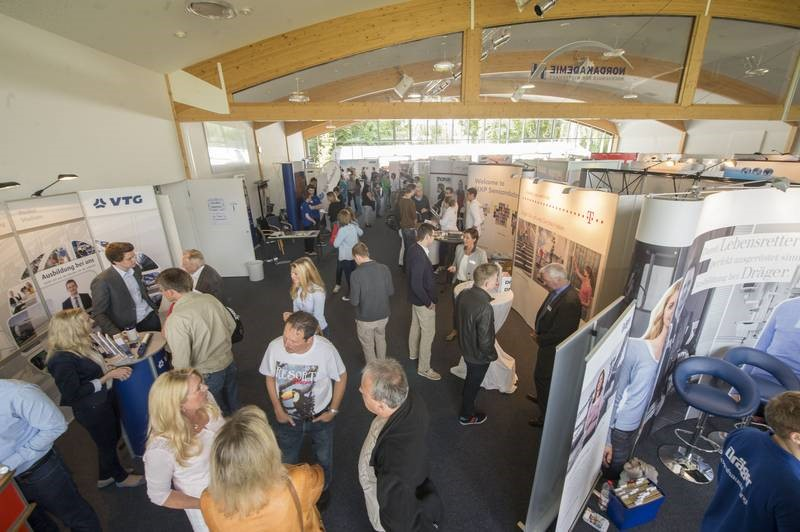
\includegraphics[width=0.9\linewidth]{image/image1}
	\caption[Nordakademie 14. Studieninformationstag]{Nordakademie 14. Studieninformationstag}
	\label{fig:image1}
\end{figure}
\section{Tabelle}
Auch Tabellen sind toll.
\begin{lstlisting}[
    caption={Testy},
    mathescape=true,showstringspaces=false,
    flexiblecolumns=true,
    tabsize=2,
    numbersep=1pt,
    numbers=left,
    xleftmargin=0.2cm,
    framerule=0pt
    ]
  import java.util.Date;
    
  val a: String = "testy"
    
  /*
  * Bildet vereinfacht eine Person mittels einer Datenklasse in Kotlin ab.
  */

  @Testy 
  data class Person(var vorname: String, var nachname: String, 
                      var alter: Int, var geburtsdatum: Date)    
\end{lstlisting}

\begin{table}[htbp]
	\centering
    \begin{tabular}{|l|l|l|}
    \hline
    Überschrift1 & 2 & 3 \\ \hline
    ef &  & dfdf \\ \hline
    dfg & f & fgb \\ \hline
    gfp & fg &  \\ \hline
    f &  &  \\ \hline
    juhz &  & rt \\ \hline
    rtg &  & ikiu \\ \hline
    \end{tabular}
    \caption{Beispieltabelle} 
    \label{table:Tabelle}
\end{table}

\chapter{Glossar}
Es wird zwischen Worterklärungen (Glossar) und Abkürzungen (Akronymen) unterschieden.
\section{Glossar}
Dies ist ein Beispiel für ein Eintrag im \Gls{glossar}. Das Wort kann auch im Plural ausgegeben werden (\Glspl{glossar}).
\section{Akronyme}
\gls{latex} wird automatisch bei der ersten Nutzung des Akronyms die Erklärung hinzufügen. Bei späteren Erwähnungen wird \gls{latex} nur die Abkürzung ausgeben.
\chapter{Literatur}
Es kann ganz einfach auf eine Quelle verwiesen werden \autocite{blubb}